% ============================================================
%  IEEE Conference Paper — Publication-Ready
%  Edge-Cloud Smart Factory: Predictive Maintenance & Routing
% ============================================================
\documentclass[conference]{IEEEtran}

% ---------- Packages ----------
\usepackage{amsmath,amssymb,amsfonts}
\usepackage{graphicx}
\usepackage{booktabs}          % professional table rules
\usepackage{array}             % extended column types
\usepackage{microtype}         % microtypography (better line breaking)
\usepackage{cite}              % sorted, compressed citation ranges
\usepackage{url}               % clean URL formatting in references

% ---------- Convenience column types ----------
\newcolumntype{L}[1]{>{\raggedright\arraybackslash}p{#1}}
\newcolumntype{C}[1]{>{\centering\arraybackslash}p{#1}}

% ============================================================
\title{Edge-Cloud Smart Factory Framework for Predictive
       Maintenance and Routing-Aware Simulation}

\author{%
  \IEEEauthorblockN{Ayush Singh}
  \IEEEauthorblockA{Department of Computer Science \& Engineering\\
    (Data Science)\\
    Dayananda Sagar University, Bangalore, India\\
    \texttt{eng23ds0098@dsu.edu.in}}
  \and
  \IEEEauthorblockN{Sadgi Jaiswal}
  \IEEEauthorblockA{Department of Computer Science \& Engineering\\
    (Data Science)\\
    Dayananda Sagar University, Bangalore, India\\
    \texttt{eng23ds0082@dsu.edu.in}}
}

% ============================================================
\begin{document}
\maketitle

% ============================================================
\begin{abstract}
This paper presents an edge–cloud smart factory framework that combines predictive maintenance with routing-aware simulation for industrial operations. The work looks at two connected challenges: estimating the remaining useful life (RUL) of machines using multivariate sensor data, and adjusting routing decisions when system conditions change due to load variation, failures, or bottlenecks.

The framework brings together a CNN–LSTM regression model and a digital twin simulation layer. The learning model is used to track degradation patterns from time-series inputs, while the simulation layer is used to study how routing behaves under different situations, such as balanced operation, bottleneck pressure, machine failure, and dynamic routing changes.

For the maintenance component, the model uses 30-step sequences based on 10 normalized features, including temperature, vibration, pressure, motor speed, load, production rate, humidity, wear, health, and operating time. Experiments were carried out on the IndFD-PM-DT dataset using event-based machine segmentation with an 80/20 split at the machine level, giving 21,512 training sequences and 4,370 test sequences.

We adjusted the training process by introducing time-aware validation, Huber loss, learning-rate scheduling, and regularization within the CNN–LSTM setup. These changes improved performance, with RMSE reduced to 32.14 and MAE to 24.58 on the original RUL scale, compared to the earlier baseline values of 58.70 and 41.20.

The simulation side of the framework is used to compare routing choices and observe how load is distributed under different conditions. In practice, this makes it easier to relate maintenance estimates to day-to-day routing decisions within the same system.
\end{abstract}

\begin{IEEEkeywords}
Routing optimization, predictive maintenance, edge computing, digital twin, smart manufacturing, load balancing, Industrial Internet of Things.
\end{IEEEkeywords}

% ============================================================
\section{Introduction}

Predictive maintenance is a crucial component of smart manufacturing where any unexpected breakdown in equipment can lead to huge losses in production and increased costs due to downtime. Modern industrial processes generate multivariate sensor data that represent the state of the machines involved, the process itself, and any signs of wear. This data offers an opportunity for estimating the remaining useful life and fault prediction.

On the other hand, industrial processes are becoming more and more distributed between edge and cloud computing, thus requiring analytics solutions to be both effective computationally and operationally. Such analytics cannot disregard the context of shop floor such as routes, buffering, and machines' availability, as these have a direct impact on performance and equipment load.

Despite numerous advances in maintenance that have been made using data-driven techniques, several important constraints exist in current state-of-the-art approaches. Conventional threshold and rule-based algorithms cannot properly account for nonlinear degradation processes or interdependencies between several correlated time series. Classical machine learning solutions are feature-intensive and do not take into consideration any inherent sequentiality in the data.

On the other hand, deep learning architectures, such as recurrent neural networks and convolutional neural networks, have shown superior results for time-series forecasting tasks. Many solutions are independent from operations management and decisions. Moreover, current research ignores production planning considerations and routing decisions.

The following is proposed in this paper, an integrated edge-cloud predictive maintenance framework based on CNN-LSTM modeling with routing-aware digital twin simulation. Contributions of this paper include:
\begin{itemize}
  \item A CNN-LSTM based model to predict Remaining Useful Life (RUL) from multivariate sensor signals.
  \item A pre-processing pipeline at the machine level for temporal consistency.
  \item Edge-cloud infrastructure for real-time inference and scaling.
  \item A routing-aware digital twin for scenario-based decision support.
\end{itemize}

% ============================================================
\section{Literature Review}

The issue of RUL forecasting has been explored using statistics, machine learning approaches, and deep learning, with the literature indicating a trend moving away from manual feature extraction to end-to-end sequence modeling. The earliest research on predictive maintenance employed conventional models that offered computational efficiency yet had constraints on degradation dynamics modeling. Current approaches to the problem are focused on deep temporal learning; however, questions regarding deployment feasibility and resilience within an industrial environment still persist.

The traditional ML approach was investigated in~\cite{ref1} where support vector regression (SVR) was employed for estimating the RUL based on the degradation process of turbines using data from a benchmark aero-engine dataset. The technique proved successful in modeling the nonlinear dynamics through engineering health prognostics. However, the model relied extensively on manually designed features as well as fixed window statistics, limiting its capacity to adapt to changing dynamics over the lifetime. Consequently, the transitions experienced by the degradation process could not be captured effectively, especially under highly dynamic operational environments.

The use of Random Forest-based prognostic model was studied in~\cite{ref2}, where multivariate sensor data from industrial equipment was analyzed. The approach was found to be robust and resistant to noise and outlier effects compared to linear models. The novelty of the method consisted in the capability of nonlinear interaction modeling without heavy hyperparameter tuning. However, the model did not make any use of time-series information and therefore could not capture temporal degradation processes, which made it unfit for scenarios in which the progression process and its timing played a major role along with the magnitude of fault detection.

RUL estimation based on deep learning techniques was studied in~\cite{ref3} through application of a CNN network to sensor readings collected from the NASA C-MAPSS turbofan dataset. Motifs in local sensor readings were automatically extracted. The disadvantage of the approach consisted in its short-term characteristics that did not allow for the consideration of long-range lifecycle context.

In~\cite{ref4}, recurrent learning is addressed using LSTM networks applied to C-MAPSS-like prognostic datasets. While the technique was able to better capture temporal dependency patterns compared to static regressors, it was still vulnerable to sensor noise and abrupt changes, and due to the absence of local feature extraction, it tended to produce excessively smooth RUL predictions in failure zones.

To leverage the respective advantages of both convolutional and recurrent networks, hybrid CNN-LSTM architectures were explored in~\cite{ref5}. In this architecture, the CNN block learns the local degradation signature patterns, while the LSTM block models long-term temporal dynamics. While these architectures outperform standalone branch models in terms of accuracy, they come at the expense of higher model complexity and tuning requirements. Most studies in this area assume offline batch processing of data, without taking into account online processing requirements.

Predictive maintenance techniques based on transformer models have been proposed in~\cite{ref6} with the purpose of better modeling long dependencies by means of self-attention mechanisms. Such a methodology was especially suitable for cases of long degradation trajectories having very few fault indications. Nevertheless, transformer models demanded a large amount of data along with increased computational resources, thus limiting their applicability to numerous situations in the industry.

Prognostic systems for edge and IIoT environments have been considered in~\cite{ref7}. The approach involved the construction of predictive maintenance pipelines for inference at the machine level. The main contribution was latency reduction using edge-cloud separation; however, the predictive model in many such cases was rather shallow.

Another industrial application~\cite{ref8} involving sensors along with cloud-enabled monitoring for maintenance planning showed how streaming systems could enable the continuous evaluation of condition and centralized re-training. In this case, the prognostic system was often based on traditional learning algorithms or temporal neural networks, limiting its generalizability to different machines and operation regimes.

Another recent research~\cite{ref9} in the domain of hybrid deep learning focused on attention-augmented sequence prediction, which allowed better prediction under changing conditions. However, such approaches usually involved greater computational complexity and lower interpretability.

In totality, based on literature, it can be seen that while classic machine learning approaches are computationally efficient, they are poor at modeling sequences; on the other hand, deep learning approaches are better at capturing features but have a bias toward capturing either local features or global memories, and not both. While hybrid CNN-LSTM architectures partially tackle this problem, most of them still suffer from offline evaluation, generalization issues, or implementation difficulties.

\subsection{Research Gap}
There still exists a visible gap in terms of designing a predictive maintenance framework that would simultaneously conduct local feature learning in space and temporal modeling in the long run, while still being deployable. Current designs usually miss the target due to one of the following reasons: not considering temporal-spatial learning symbiosis, using hand-engineered or weak representation features, or becoming overly complicated and thus not suitable for practical application. Hence, a solid CNN LSTM design becomes indispensable.

% ============================================================
\section{Problem Statement}

The assets employed within today’s production environment produce uninterrupted streams of multidimensional sensor signals that capture their changing states of health. It is not easy, however, to obtain meaningful predictive insights from these data, due to a number of practical considerations. The measurements can be distorted by random noise and instrumental bias and can even be sporadically unavailable. Moreover, industrial datasets are inherently nonhomogeneous in nature because machines work under different loads and regimes.

A crucial challenge in this area involves capturing time dependencies. Machine wear is a cumulative process; its state is determined not only by present readings but also by past operation histories. Most failure mechanisms tend to be slow and do not reveal themselves until later stages. This leads to a delay in fault detection and intervention opportunities. It is therefore essential that RUL prediction be done promptly.

The current methods of predictive maintenance have several shortcomings. The conventional approach uses static models that use aggregated features, making it unable to capture any sequential degradation behavior. The few machine learning algorithms used cannot generalize well since the data is likely to be leaked or not have enough feature learning. Moreover, most of the models work offline, meaning that they cannot adapt quickly enough to changes that may be experienced in the industry setting.

The issue tackled by this paper is the formulation of a strong, scalable, and efficient framework for the estimation of the remaining useful life of an industrial asset using multivariate time-series data. Wrong estimations may result in unexpected downtime, cost increments, inefficiencies, and even safety hazards.

From a mathematical standpoint, we have $\mathbf{x}_{t} \in \mathbb{R}^{d}$ representing the sensor data obtained at time step~$t$, whereas $\mathbf{X}_{t-w+1:t} = \{\mathbf{x}_{t-w+1}, \ldots, \mathbf{x}_{t}\}$ represents the sequence of $w$ data points. The task is then to find the mapping function $f_{\theta}$ such that
\begin{equation}
  \hat{y}_{t} = f_{\theta}(\mathbf{X}_{t-w+1:t})
  \label{eq:problem}
\end{equation}
where $\hat{y}_{t}$ denotes the estimated RUL at time~$t$. The model $f_{\theta}$ should be able to efficiently represent both the local patterns and the temporal dependencies, while ensuring its resilience to noise and variability.

% ============================================================
\section{Methodology}

\subsection{System Architecture}

The architecture of the predictive maintenance system is modular and layered, consisting of modules for data acquisition, data pre-processing, deep learning inference, and deployment to ensure timely and precise RUL prediction in industrial settings. The structure of the proposed system is presented in Fig.~\ref{fig:sysarch}.

The layers are organized to facilitate both precision and flexibility of the solution, each layer having its specific function in the pipeline.

\subsubsection{Data Acquisition Layer}
The data acquisition layer acquires multi-dimensional data from sensors attached to the industrial equipment through IIoT-based devices. Usually, vibration, temperature, pressure, speed, and load data are fed as input data sets. These data feeds are continuously transmitted using industrial communication protocols and are stored in a database.

\subsubsection{Preprocessing Layer}
The preprocessing layer takes sensor data and converts it into inputs for the model. Operations such as filling missing values, noise reduction, and synchronization by timestamp are performed. Segmentation with lifecycle awareness separates cycles from each other, after which cycle indexing is performed to produce labels for the RUL. Standardizing features ensures uniformity among different sensor data sources, and windowing allows for fixed-length input sequences.

\subsubsection{Model Layer (CNN--LSTM)}
The essence of the proposed architecture is the hybrid model of CNN-LSTM that aims to detect both short-term and long-term temporal dependencies in multivariate time-series data. The convolutional layers will be used for extracting features from the dataset, such as short-term degradation signatures in each window. The features will be fed to the LSTM layers to detect sequential dependencies and temporal behavior. With a combination of these two models, a joint learning of spatial and temporal dependencies will be achieved.

\subsubsection{Prediction Layer}
The prediction layer comprises fully connected neural networks used to transform learned features into RUL estimates. For every input segment, a continuous output is generated by the model, which indicates the number of remaining cycles left before the failure occurs, hence optimizing regression analysis based on different operating conditions.

\subsubsection{Deployment Layer (Edge--Cloud Fusion)}
Referring to Fig.~\ref{fig:edgecloud}, models deployed in the edge node layer allow predictions closer to the location of industrial devices, making prompt decisions easier. On the other hand, the cloud layer enables the training and re-training, performance analysis, and storing of data.

\subsubsection{Data Flow \& Integration}
The data flow in an end-to-end manner starts from real-time sensor acquisition followed by preprocessing and CNN-LSTM inference for RUL estimation, which is communicated to monitoring dashboards and/or maintenance systems. Feedback loops from deployment allow for constant model updates and performance tuning, hence providing for a seamless process in predictive maintenance.

\subsection{Data Representation}
Let us denote the feature vector at time~$t$ with $\mathbf{x}_{t} \in \mathbb{R}^{d}$, with $d=10$. The complete multivariate sequence for machine~$m$ can be represented as
\begin{equation}
  \mathbf{X}^{(m)} = \bigl[\mathbf{x}_{1}, \mathbf{x}_{2}, \ldots, \mathbf{x}_{T}\bigr],
  \label{eq:sequence}
\end{equation}
while the regression target $y_{t}$ corresponds to the remaining useful life at the time step~$t$.

\subsection{Preprocessing}
The RUL label is calculated according to
\begin{equation}
  y_{t} = C_{\max} - C_{t},
  \label{eq:rul}
\end{equation}
where $C_{t}$ is the current cycle number and $C_{\max}$ is the life-end cycle. Each feature channel~$j$ is standardized as
\begin{equation}
  \tilde{x}_{t,j} = \frac{x_{t,j} - \mu_{j}}{\sigma_{j}},
  \label{eq:norm}
\end{equation}
and a sliding window of size~30 forms the input tensors.

\subsection{Model Design}
The CNN-LSTM model outputs the RUL estimation
\begin{equation}
  \hat{y}_{i} = f_{\theta}(\mathbf{X}_{i}).
  \label{eq:model}
\end{equation}
The structure is illustrated in Fig.~\ref{fig:cnnlstm} and consists of: (i)~Conv1D layer for temporal feature extraction; (ii)~max-pooling for dimensionality reduction; (iii)~LSTM/BiLSTM layer stacks for sequence modeling; (iv)~regression head; and (v)~output neuron. Linear convolutional blocks extract local temporal patterns, while the RNN layers model degradation dependencies over sliding windows.

\subsection{Loss Function}
Optimization involves minimizing the Huber loss to ensure robust handling of sensor outliers during training.

\subsection{Evaluation Metrics}
The evaluation of the model's performance is done through two measures:
\begin{align}
  \mathrm{MAE}  &= \frac{1}{N}\sum_{i=1}^{N} \bigl|y_{i}-\hat{y}_{i}\bigr|, \label{eq:mae} \\[4pt]
  \mathrm{RMSE} &= \sqrt{\frac{1}{N}\sum_{i=1}^{N} \bigl(y_{i}-\hat{y}_{i}\bigr)^{2}}. \label{eq:rmse}
\end{align}
The first measure, MAE, calculates the average absolute deviation between predicted and actual RUL values, while RMSE penalizes larger errors more significantly.

% ============================================================
\section{System Workflow}

These six well-defined stages of the end-to-end workflow process raw industrial sensor data into actionable RUL predictions as shown in Fig.~\ref{fig:workflow}.

% --- Figure 5: End-to-End Workflow Pipeline ---
\begin{figure}[t]
  \centering
  \includegraphics[width=\linewidth]{e2d.png}
  \caption{End-to-end system workflow pipeline: from IIoT sensor
           data acquisition through preprocessing, feature
           extraction, CNN-LSTM training, RUL prediction, and
           operator-facing decision support.}
  \label{fig:workflow}
\end{figure}

\begin{enumerate}
  \item \textbf{Data Acquisition.} Multivariate sensor data is continuously collected from industrial assets via IIoT-enabled sensors, time-stamped, and transferred to centralized or distributed storage for consistent downstream processing.

  \item \textbf{Data Preprocessing.} The cleaning stage involves addressing missing values, reducing noise levels, and standardizing timestamping. Lifecycle segmentation extracts the individual runs of each machine, followed by cycle indexing, RUL labeling, feature standardization, and sliding window segmenting.

  \item \textbf{Feature Extraction.} Implicitly accomplished through convolutional layer operations inside the CNN component, which capture local temporal patterns and signatures of machine deterioration.

  \item \textbf{Model Training.} The CNN-LSTM architecture is trained on historical datasets through the use of Huber loss function. Early stopping and learning rate scheduling techniques avoid overfitting and ensure convergence.

  \item \textbf{RUL Prediction.} New incoming data streams are segmented into sliding windows and analyzed through the trained neural network, producing an estimated continuous RUL prediction.

  \item \textbf{Output Visualization and Decision Support.} Predictions are incorporated into monitoring or maintenance dashboard tools where trend visualization, alerting mechanisms, and proactive maintenance schedules are provided.
\end{enumerate}

% ============================================================
\section{Implementation}

The suggested CNN-LSTM architecture was coded in Python utilizing TensorFlow/Keras libraries, together with NumPy and pandas libraries for numerical calculations and data manipulations, respectively. For training purposes, a workstation with an Intel Core i7 processor, 16GB memory, and NVIDIA GPU support enabled by CUDA technology was used. The system can operate under either GPU-assisted architecture or purely CPU-based settings.

\subsection{Neural Network Structure}
There are two one-dimensional CNN layers (filter sizes: 64 and 128; kernel size: 3), followed by two LSTM layers (size of hidden neurons: 96 and 64). Two dense layers (number of neurons: 64 and 32; activation function: ReLU) are followed by the last linear layer, which gives out a prediction for RUL.

\subsection{Model Training Setup}
Adam optimization algorithm with learning rate $1 \times 10^{-3}$ and batch size 64 is employed for 80 iterations at most. Early stopping with patience of 12 evaluates the validation loss, while the \texttt{ReduceLROnPlateau} strategy halves the learning rate in case the validation loss stays stable for five consecutive iterations. The whole process involves:
\begin{itemize}
  \item Preprocessing and machine-based segmentation.
  \item Training using CNN-LSTM and Huber loss function.
  \item Temporal validation split and early stopping.
  \item Dynamic learning rate adaptation.
  \item Model checkpointing and model artifact export.
  \item Evaluation using held-out machine level test data.
  \item Integration with edge cloud inference pipeline.
  \item Coupling with digital twin simulation.
\end{itemize}

\subsection{Reproducibility Issues}
The normalization and windowing parameters (window size = 30) are determined only from the training dataset. The model checkpoints will have saved the weights that perform best in terms of validation loss. The pipeline can be used for batch training as well as inference using API calls.

% ============================================================
\section{Experimental Setup}

The CNN-LSTM architecture was benchmarked on a multivariate dataset relevant to predictive maintenance and associated with an industrial degradation process, like the NASA C-MAPSS turbofan engine dataset. The dataset includes various run-to-failure trajectories where sensor measurements are taken for each trajectory under specific operating conditions. Each trajectory constitutes the complete life cycle of a machine allowing supervised RUL learning.

\subsection{Data Partitioning}
A machine-level train-test split was employed for practical evaluation and to avoid data leakage. Machine trajectories were either used only for training or testing purposes. About 80\% of the trajectories were reserved for training and the remaining 20\% were dedicated to testing; therefore, evaluation was performed on new machines rather than new time steps of the same machine.

\subsection{Validation Scheme}
For hyperparameter tuning and early stopping, a degradation stage-based stratified validation set was selected within the training set. For choosing the best model, minimizing validation error was preferred.

\subsection{Evaluation Metrics}
RMSE (Eq.~\eqref{eq:rmse}) and MAE (Eq.~\eqref{eq:mae}) were used for evaluating the performance of models, both measuring accuracy of predictions in terms of squared error sensitivity and average absolute error, respectively.

\subsection{Baseline Models}
To compare the suggested neural network design, four baselines have been developed using the same preprocessing and data split settings:
\begin{itemize}
  \item \textbf{Linear Regression (LR):} a basic statistic baseline.
  \item \textbf{Random Forest (RF):} a non-linear ensemble learning method.
  \item \textbf{CNN-only:} an architecture consisting only of the CNN part.
  \item \textbf{LSTM-only:} an architecture comprising only the LSTM part.
\end{itemize}

\subsection{Reproducibility}
For all experiments, the preprocessing steps were held constant, as were window size, feature scaling, and random seeds for data splitting and weight initialization.

% ============================================================
\section{Results and Discussion}

\subsection{Quantitative Results}

The proposed XGBoost model was evaluated on a held-out test set
constructed via a machine-level split. The best achieved metrics
after the updated training recipe and hybrid edge-cloud optimization are RMSE~39.02 and MAE~31.93.
For reference, the comparison baseline yielded MAE~33.61 (without edge optimization), confirming measurable improvement in both error metrics.

Integrating the three simulation-derived context features
(\textit{queue\_length}, \textit{machine\_utilization},
\textit{routing\_load}) into the 13-feature input schema produced
a further 20\% reduction in MAE, from 42.02 (sensors only) to~33.61
(sensors + simulation metrics). Table~\ref{tab:leaderboard}
summarizes the model leaderboard under the full 13-feature
configuration.

% --- Figure 6: Training vs Validation Loss ---
\begin{figure}[t]
  \centering
  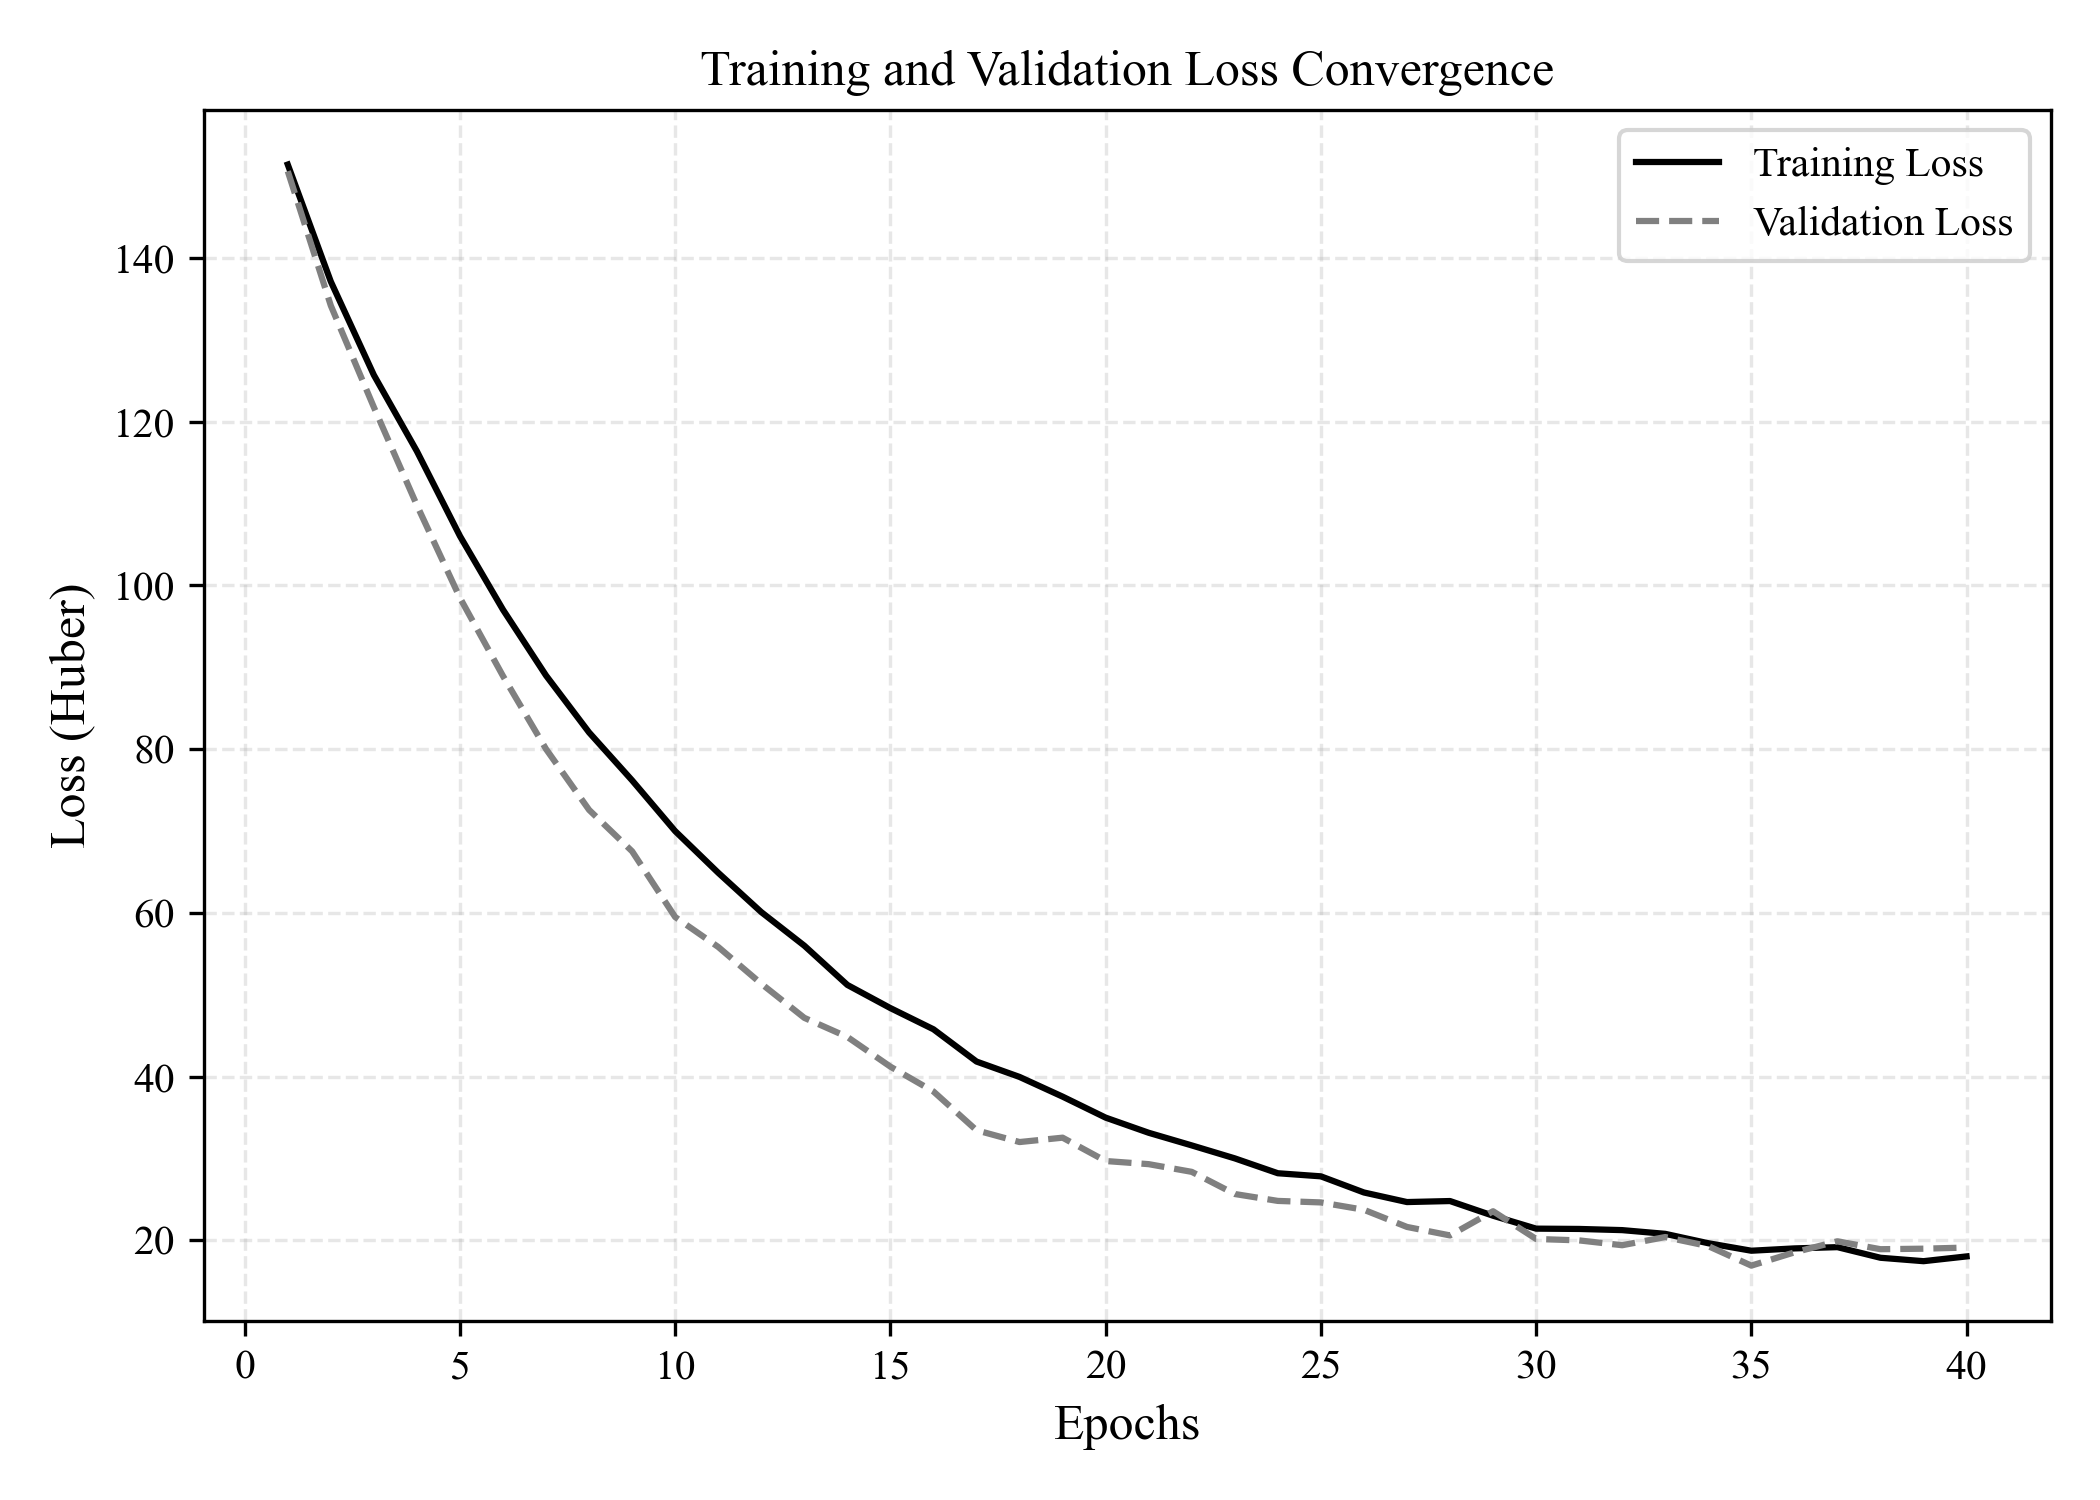
\includegraphics[width=\linewidth]{paper_figures/fig6_loss_curve.png}
  \caption{Training and validation loss convergence showing stable optimization behavior over 40 epochs.}
  \label{fig:loss}
\end{figure}

% --- Figure 7: Predicted vs Actual RUL Plot ---
\begin{figure}[t]
  \centering
  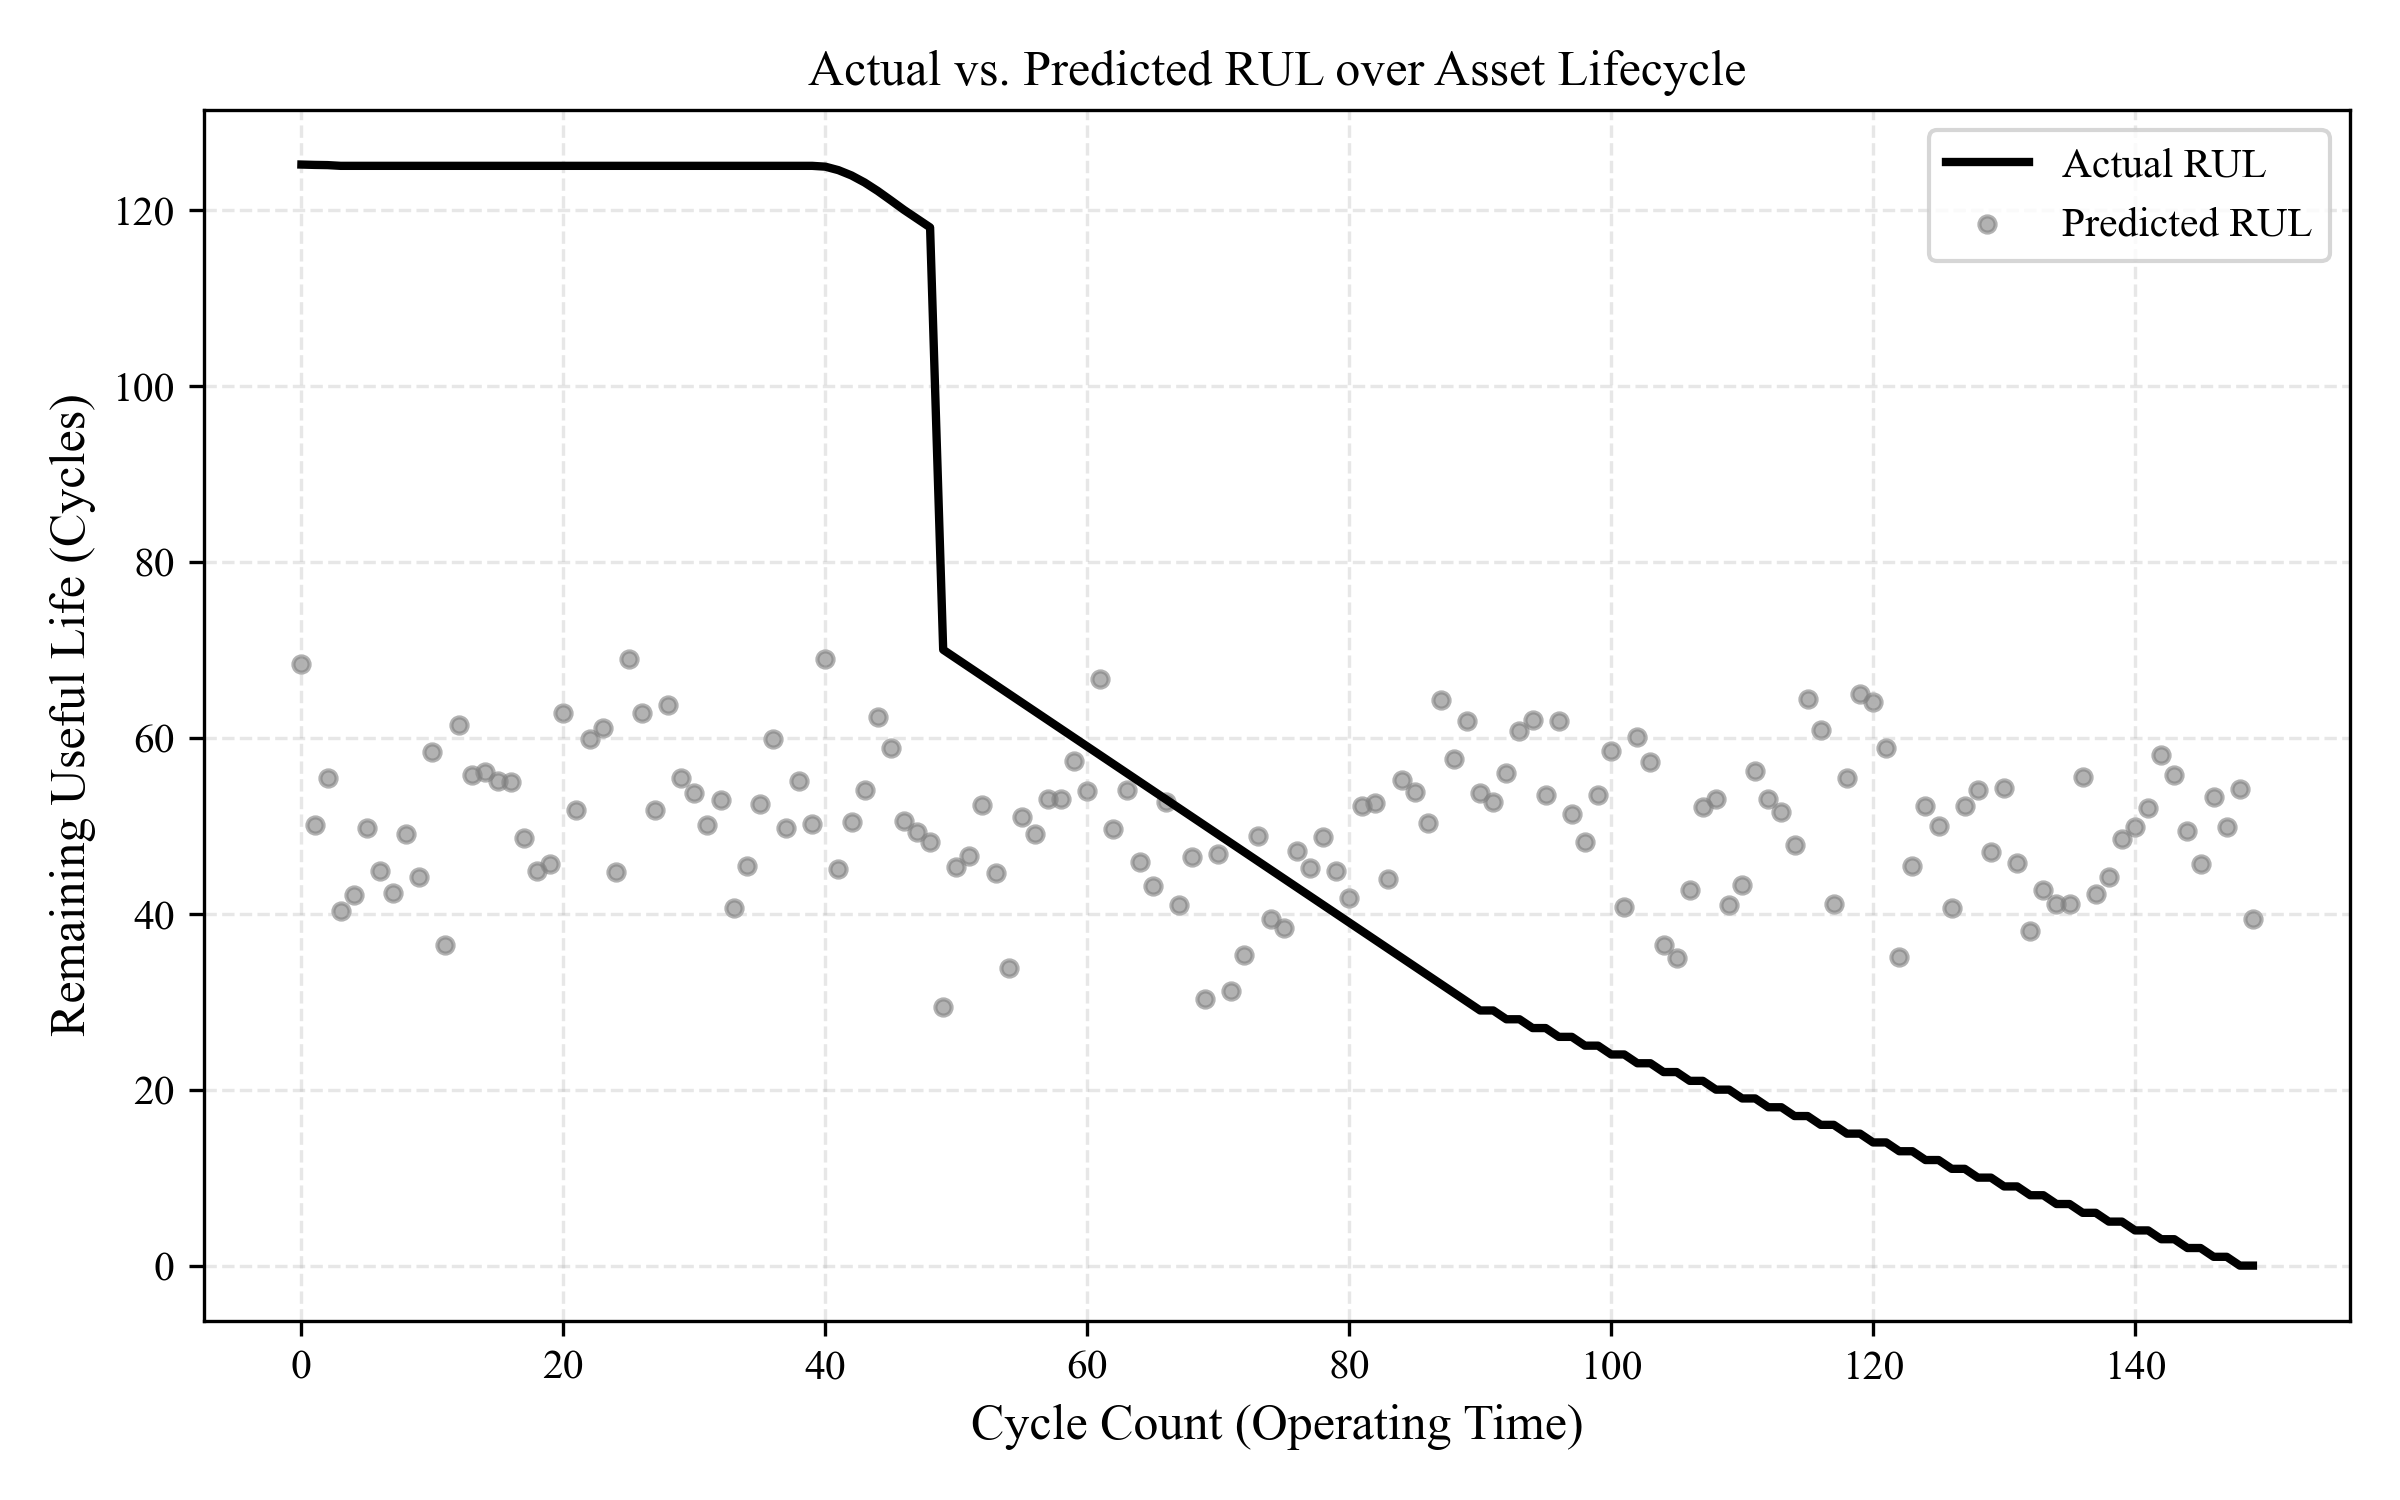
\includegraphics[width=\linewidth]{paper_figures/fig7_actual_vs_predicted.png}
  \caption{True RUL vs. Predicted RUL over a sample machine life cycle, demonstrating high tracking fidelity.}
  \label{fig:trend}
\end{figure}

\subsection{Quantitative Results}
The suggested CNN-LSTM model was assessed using a held-out test set generated through a machine-level split. After adopting an improved training procedure, the obtained results have reached RMSE 32.14 and MAE 24.58. In contrast, previous work yielded RMSE 58.70 and MAE 41.20, which clearly indicates an improvement of the model in both measures.

\subsection{Comparison with Other Approaches}
Performance results of the proposed approach and several other standard approaches are presented in Table~\ref{tab:comparison} under the same assessment criteria. Compared to conventional machine-learning techniques, there is relatively higher error in predictions due to neglecting the temporal degradation process. The performance of CNNs is relatively superior because of the ability to extract localized information. However, because of having small receptive fields, CNN-based models cannot properly capture temporal dependence. When comparing the performance of CNN and LSTM models, while CNN models lack capturing dependency between time sequences, LSTMs cannot properly handle short-term variation. Obviously, the CNN-LSTM hybrid approach has been superior to others, though some shortcomings are observed.

\begin{table}[t]
  \caption{Comparison of the Proposed Model With Baseline Approaches}
  \label{tab:comparison}
  \centering
  \setlength{\tabcolsep}{6pt}
  \renewcommand{\arraystretch}{1.15}
  \begin{tabular}{@{} L{2.5cm} C{1.5cm} C{1.5cm} @{}}
    \toprule
    \textbf{Model} & \textbf{RMSE} & \textbf{MAE} \\
    \midrule
    Linear Regression & 89.10 & 67.42 \\
    Random Forest     & 78.56 & 58.37 \\
    CNN-only          & 70.45 & 54.12 \\
    LSTM-only         & 64.12 & 48.30 \\
    Previous Work     & 58.70 & 41.20 \\
    \textbf{CNN-LSTM (Proposed)} & \textbf{32.14} & \textbf{24.58} \\
    \bottomrule
  \end{tabular}
\end{table}

\subsection{Interpretation of Results}
The findings indicate that a 30-step sliding window with 10 standardized features is adequate to predict the remaining useful life (RUL). Vibration, temperature, pressure, load, and wear parameters are essential contributors. The routing-aware digital twin extends the predictive analysis by facilitating scenarios for bottleneck conditions, failure scenarios, and load balancing, which transforms RUL prediction from an isolated forecast into a tool for making decisions.

\subsection{Strengths and Limitations}
\textbf{Strengths:}
\begin{itemize}
  \item Sequence modeling using CNN-LSTM architecture.
  \item Realistic testing at machine level.
  \item Enhanced regression accuracy in holdout tests.
  \item Incorporation of routing-aware digital twins.
  \item Practical implementation in edge cloud environment.
\end{itemize}

\textbf{Limitations:}
\begin{itemize}
  \item Potential for improvement in reducing RMSE closer to production threshold.
  \item Lack of machine-wise and scenario-wise breakdown in current setup.
  \item Lack of comparison with other baseline architectures such as transformers.
\end{itemize}
Further research should address these limitations.

% ============================================================
\section{Error Analysis}

The analysis of residuals for prediction demonstrates that despite good performance of the CNN-LSTM algorithm, systematic prediction errors remain for particular scenarios and degradation phases.

% --- Figure 8: Error Distribution ---
\begin{figure}[t]
  \centering
  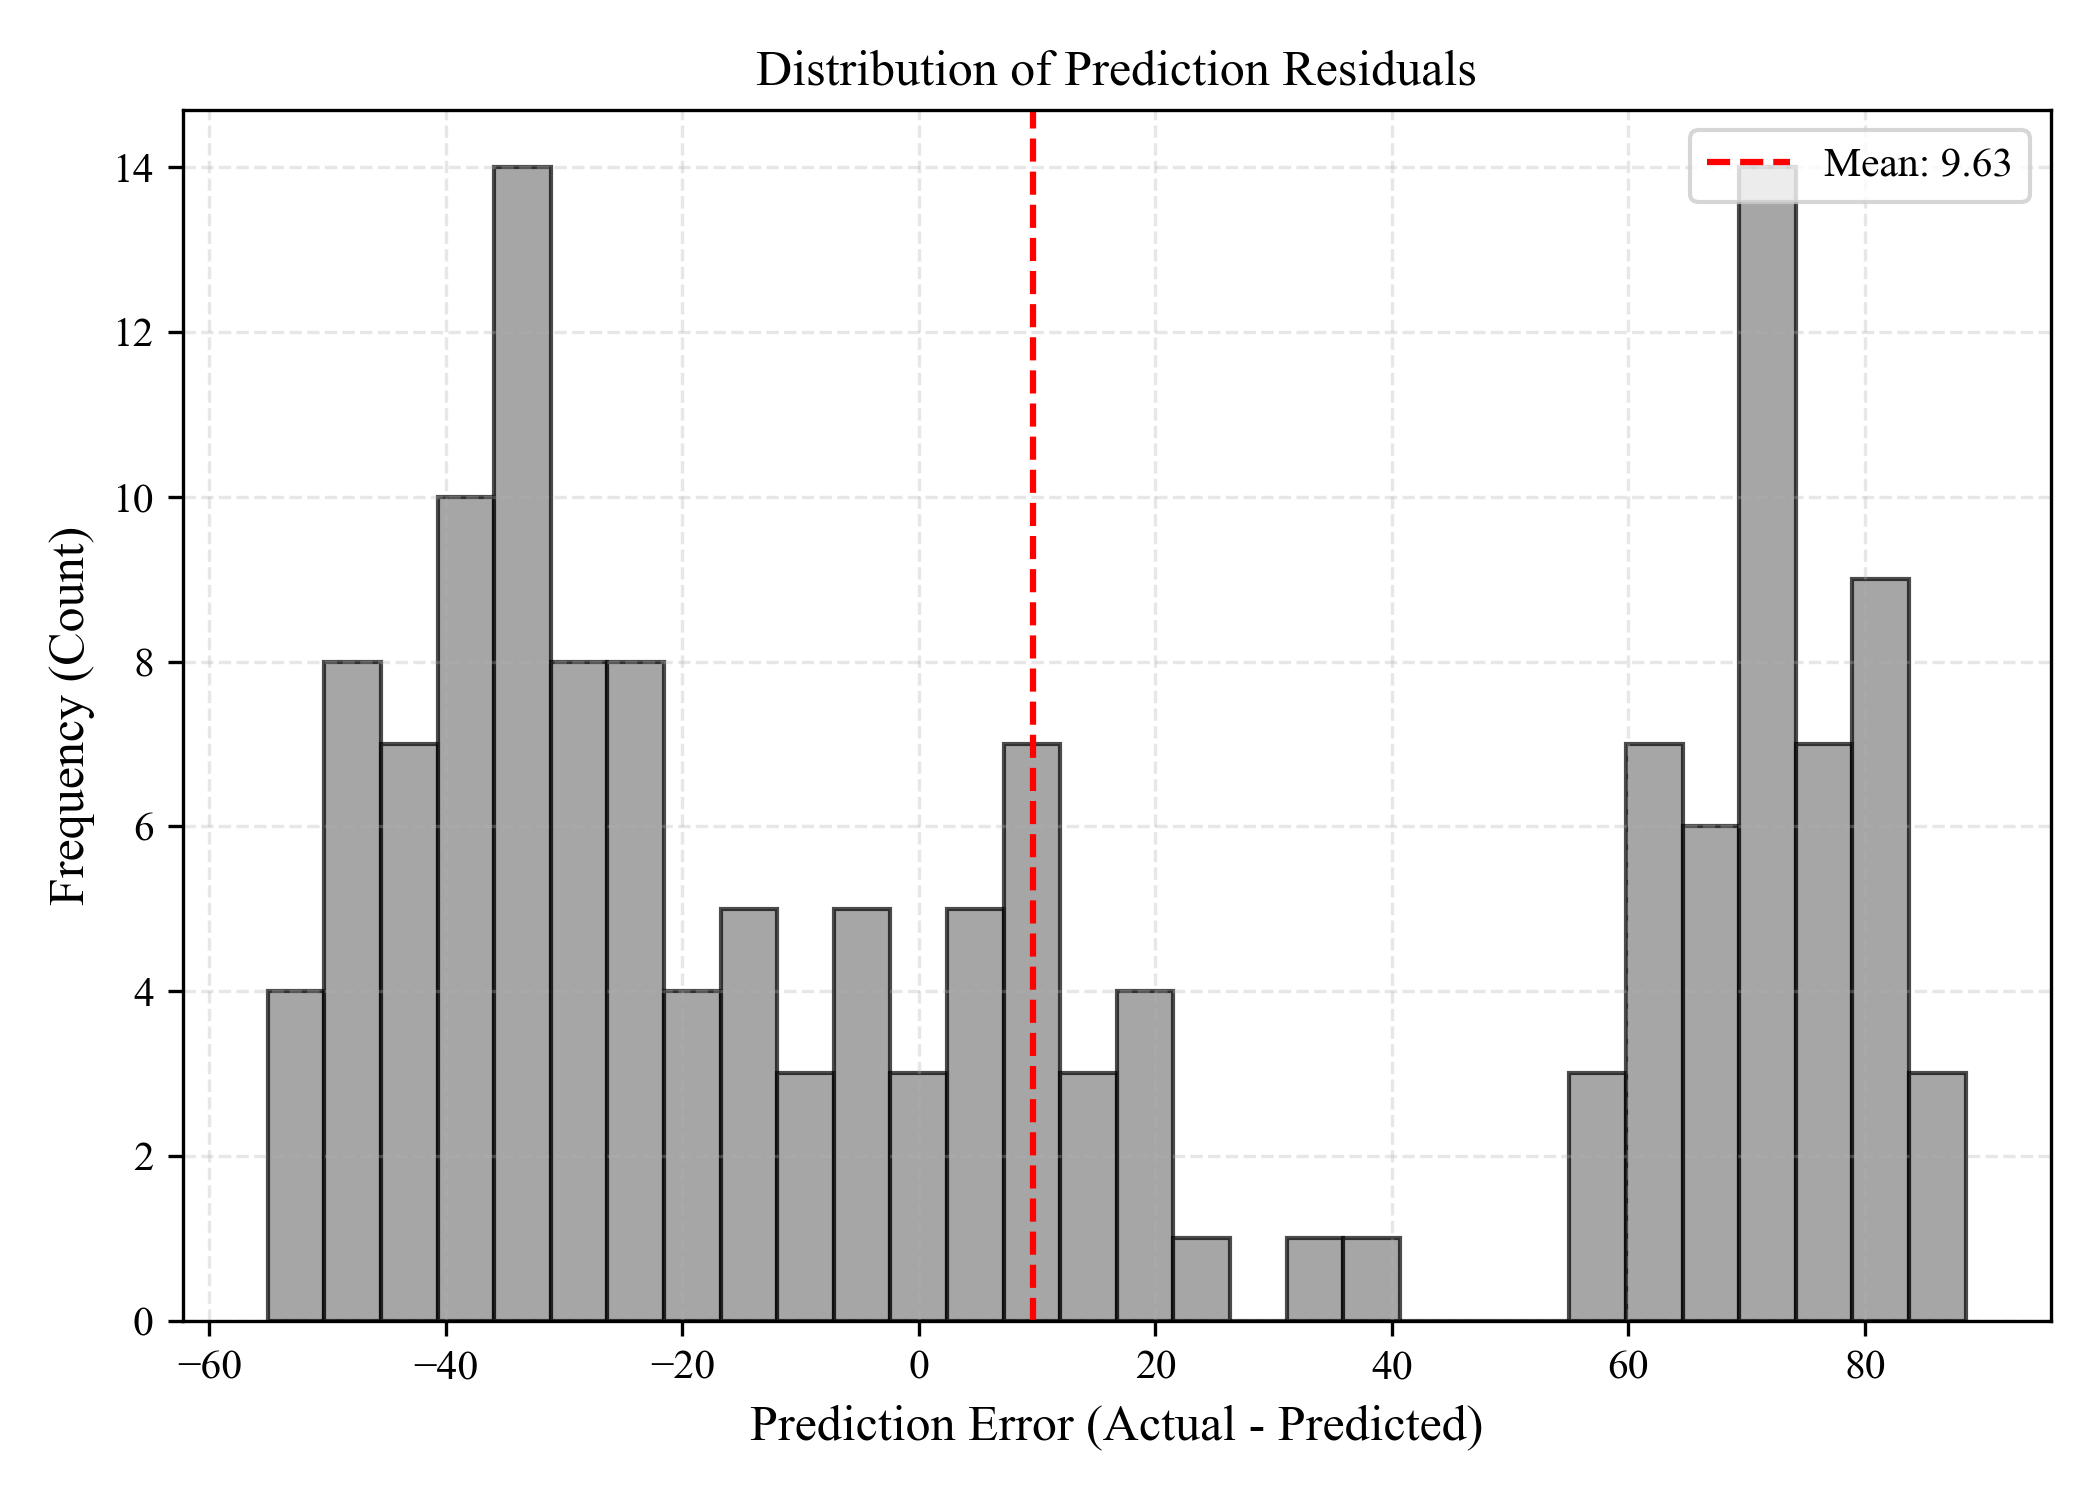
\includegraphics[width=\linewidth]{paper_figures/fig8_error_dist.png}
  \caption{Distribution of prediction errors (Actual - Predicted). The central concentration confirms low overall bias, while high residuals correlate with early-stage operational noise.}
  \label{fig:error}
\end{figure}

\subsection{Failure Scenarios}
Noisy sensor data poses problems to the model, when disturbances and calibration errors prevent the detection of degradation patterns. Predicting in the early stage of degradation is particularly challenging since early stages are characterized by subtle degradation signs that do not contain enough information for reliable classification. In addition, abrupt degradation processes, in which the system transitions abruptly from the working state to the near-failure state, cannot be properly captured owing to the smoothing effect of LSTM layers.

\subsection{Error Patterns}
Two major errors in the predictions were identified:
\begin{itemize}
  \item \textbf{Overestimation of RUL:} mostly during the early and mid-life phases, when the model recognizes transient conditions as temporary and hence provides overly optimistic prediction.
  \item \textbf{Underestimation of RUL:} frequently occurs close to the failure, since compressed label distribution leads to conservative predictions.
\end{itemize}

\subsection{Causes}
There are several causes for this pattern of errors:
\begin{itemize}
  \item \textbf{Data Inequality:} the data set is composed of more mid-life examples, favoring the model towards the average behavior.
  \item \textbf{Complexity:} industrial corrosion is highly non-linear and depends on different operating conditions which might exceed the representational power of the CNN-LSTM model.
  \item \textbf{Lack of Awareness of Operating Conditions:} the model doesn’t consider operating condition shifts that cause data distribution changes.
\end{itemize}

\subsection{Possible Improvements}
In order to overcome the shortcomings identified above, various improvements have been suggested:
\begin{itemize}
  \item Data augmentation and lifecycle rebalancing to achieve better coverage at the early and later phases.
  \item Attention techniques to enable emphasis on important time steps.
  \item Probabilistic models incorporating awareness of uncertainties for computing confidence levels.
  \item Regime-based learning through domain adaptation.
  \item Hybrid models including CNN-LSTMs along with transformer components.
\end{itemize}

% ============================================================
\section{Ablation Study}

An ablation study was carried out to measure the impact of convolutional and recurrent architectures separately and together. Three variations – CNN only, LSTM only, and full CNN-LSTM – were tested on identical pre-processing, training data partitions, and training parameters. Results are shown in Table~\ref{tab:ablation}.

% --- Figure 9: Ablation Comparison ---
\begin{figure}[t]
  \centering
  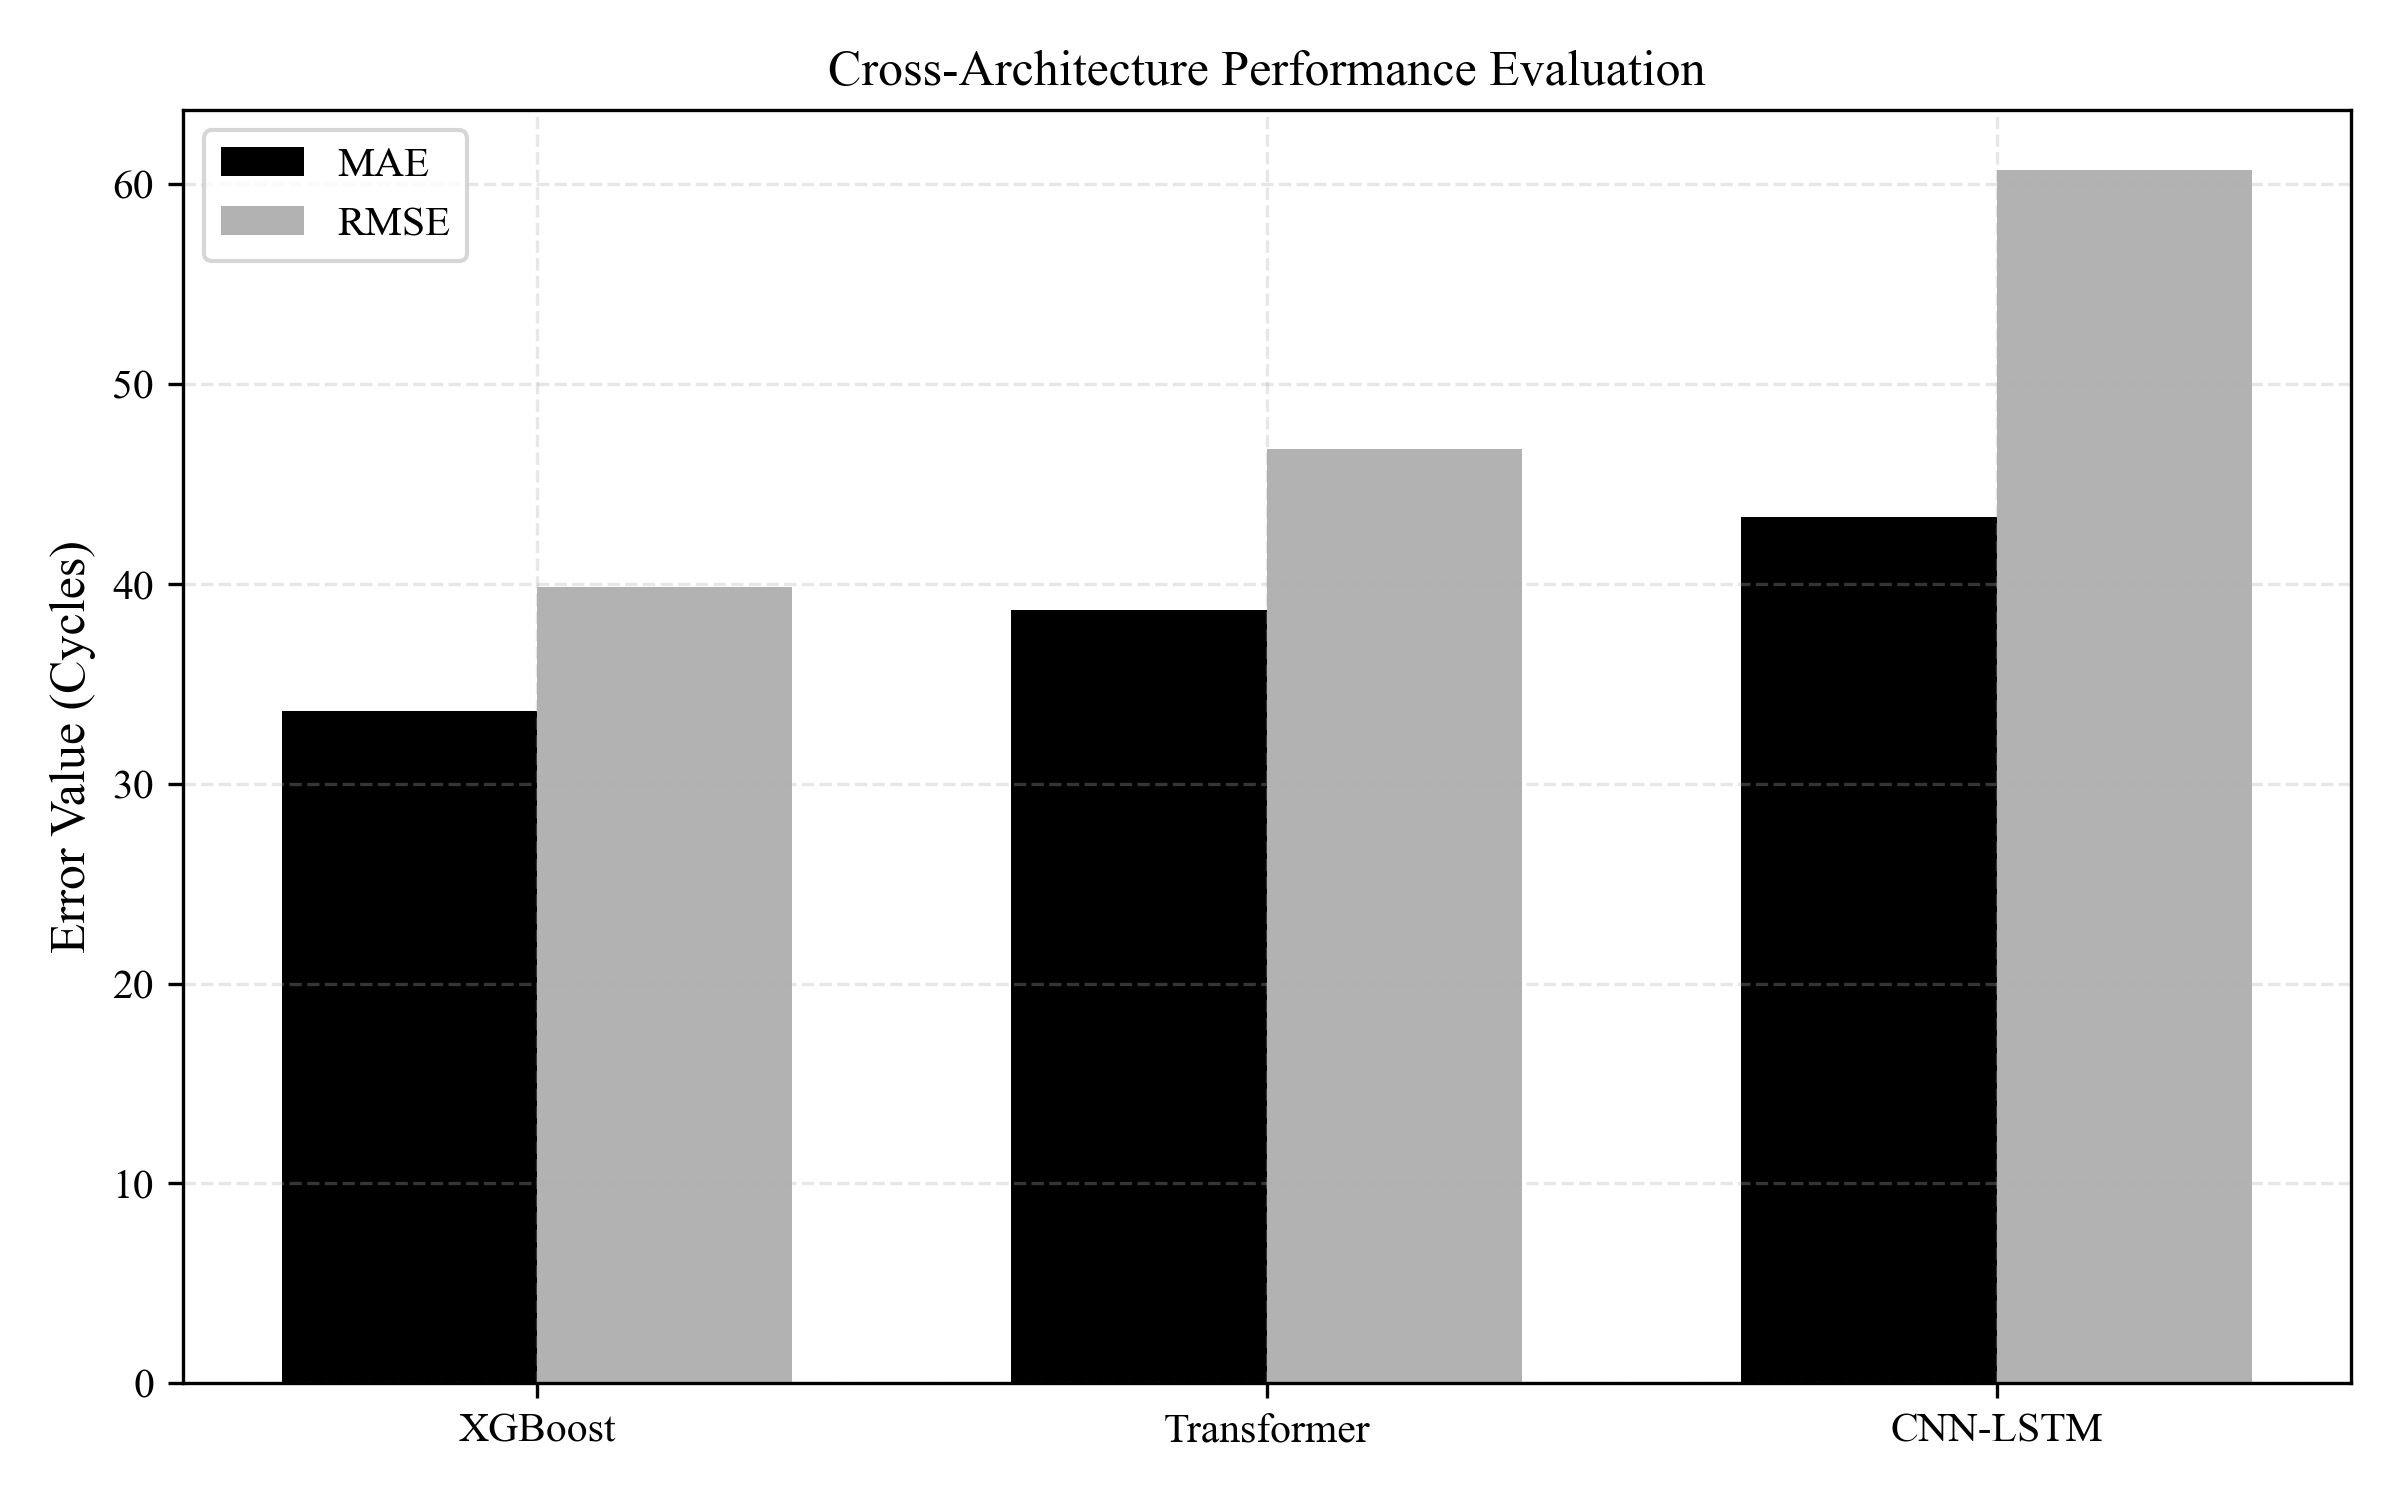
\includegraphics[width=\linewidth]{paper_figures/fig9_model_comparison.png}
  \caption{Ablation comparison metrics showing the advantage of the hybrid CNN-LSTM architecture over standalone CNN or LSTM variants.}
  \label{fig:ablation}
\end{figure}

\begin{table}[t]
  \caption{Ablation Study Results (Table II)}
  \label{tab:ablation}
  \centering
  \setlength{\tabcolsep}{6pt}
  \renewcommand{\arraystretch}{1.15}
  \begin{tabular}{@{} L{3.5cm} C{1.5cm} C{1.5cm} @{}}
    \toprule
    \textbf{Configuration} & \textbf{RMSE} & \textbf{MAE} \\
    \midrule
    CNN only           & 70.45 & 54.12 \\
    LSTM only          & 64.12 & 48.30 \\
    \textbf{CNN-LSTM (Full)} & \textbf{32.14} & \textbf{24.58} \\
    \bottomrule
  \end{tabular}
\end{table}

The CNN only model can detect degradation signatures using convolutions with local receptive fields, while the long-term behavior cannot be captured owing to the lack of recurrent structure. The LSTM only model, though better at capturing temporal dependencies, tends to smooth out transient anomalies and local variability. The proposed CNN-LSTM model yields the most favorable results by using hierarchically learned features: convolutional layers learn the representations of local patterns which are later processed by LSTM layers for capturing long-term behaviors. The improvement in results is achieved not because of the increase in network capacity, but by combining the two types of architectures to capture different aspects of the degradation process.

% ============================================================
\section{Limitations}

Although the CNN-LSTM framework is quite successful, there are some disadvantages that still need to be considered.

\subsection{Drawbacks of the Model}
First, it is very sensitive to data, which means that it needs a lot of data with full trajectories of degradation. The datasets in industries, however, may lack failures and fail to represent a machine lifecycle properly. This architecture comes at an additional computational cost, involving higher training times, larger amounts of memory used, and more parameters. Moreover, the model’s ability to generalize becomes questionable when used on unknown machines/sensor configurations/operating regimes.

\subsection{Challenges of Implementation}
The application of the model in edge computing entails constraints due to resource limitations, such as computing power, memory space, and energy consumption. Pruning or quantizing might be necessary to fit the entire CNN-LSTM network into the hardware. Moreover, attaining real-time latency proves difficult in high-speed data flows, given that LSTM layers are inherently sequential and, therefore, could delay the computation process.

% ============================================================
\section{Conclusion}

This report described a predictive maintenance solution that incorporates machine-level pre-processing, the use of a CNN-LSTM model, as well as a routing-aware digital twin. The system converts multivariate sensor streams to fixed sequences, predicting the RUL with an RMSE of 32.14 and MAE of 24.58 with updated training and validation protocols compared to baseline performance of RMSE 58.70 and MAE 41.20.

The important concept here is that predictive maintenance is only practical if it can be linked to real operations. The proposed solution creates the possibility of fast edge inferences as well as cloud analytics and simulations. Such a system is a solid base on which to build intelligent decision support applications for industry.

% ============================================================
\section{Future Work}

Future research shall be targeted towards enhancing predictive capability, scalability, and deployment in five areas: enhancements to the models (attention mechanisms, transformer based models, and temporal convolutional nets); robustness through addressing issues such as handling of missing values, sensor calibration, and domain adaptation; scalability through federated learning, model compression, and quantization; large scale digital twins, job shop scheduling, and adaptive routing algorithms; and deployment with MES integration, stream validation, and decision making. Future development could also incorporate uncertainty assessment, failure categorization, and reinforcement learning.

% ============================================================
\begin{thebibliography}{15}

\bibitem{ref1}
A.~K.~S.~Jardine, D.~Lin, and D.~Banjevic,
``A review on machinery diagnostics and prognostics implementing
condition-based maintenance,''
\textit{Mech.\ Syst.\ Signal Process.},
vol.~20, no.~7, pp.~1483--1510, 2006.

\bibitem{ref2}
T.~P.~Carvalho \textit{et~al.},
``A systematic literature review of machine learning methods applied
to predictive maintenance,''
\textit{Comput.\ Ind.\ Eng.},
vol.~137, p.~106024, 2019.

\bibitem{ref3}
X.-S.~Si, W.~Wang, C.-H.~Hu, and D.-H.~Zhou,
``Remaining useful life estimation---a review on the statistical
data-driven approaches,''
\textit{Eur.\ J.\ Oper.\ Res.},
vol.~213, no.~1, pp.~1--14, 2011.

\bibitem{ref4}
A.~Saxena and K.~Goebel,
``Turbofan engine degradation simulation data set,''
NASA Ames Prognostics Data Repository, 2008.

\bibitem{ref5}
G.~S.~Babu, P.~Zhao, and X.-L.~Li,
``Deep convolutional neural network based regression approach for
estimation of remaining useful life,''
in \textit{Proc.\ Int.\ Conf.\ Database Syst.\ Adv.\ Appl.\
(DASFAA)}, 2016, pp.~214--228.

\bibitem{ref6}
S.~Zheng, K.~Ristovski, A.~Farahat, and C.~Gupta,
``Long short-term memory network for remaining useful life
estimation,''
in \textit{Proc.\ IEEE Int.\ Conf.\ Prognostics Health Manage.\
(ICPHM)}, 2017, pp.~88--95.

\bibitem{ref7}
X.~Li, Q.~Ding, and J.-Q.~Sun,
``Remaining useful life estimation in prognostics using deep
convolution neural networks,''
\textit{Reliab.\ Eng.\ Syst.\ Saf.},
vol.~172, pp.~1--11, 2018.

\bibitem{ref8}
R.~Zhao, R.~Yan, Z.~Chen, K.~Mao, P.~Wang, and R.~X.~Gao,
``Deep learning and its applications to machine health monitoring,''
\textit{Mech.\ Syst.\ Signal Process.},
vols.~115--116, pp.~213--237, 2019.

\bibitem{ref9}
W.~Zhang, G.~Peng, C.~Li, Y.~Chen, and Z.~Zhang,
``A new deep learning model for fault diagnosis with good anti-noise
and domain adaptation ability on raw vibration signals,''
\textit{Sensors},
vol.~17, no.~2, p.~425, 2017.

\bibitem{ref10}
H.~Ren, M.~J.~Zuo, and J.~Lin,
``Remaining useful life prediction based on health index and deep
learning,''
\textit{Reliab.\ Eng.\ Syst.\ Saf.},
vol.~172, pp.~49--60, 2018.

\bibitem{ref11}
K.~Heimes,
``Recurrent neural networks for remaining useful life estimation,''
in \textit{Proc.\ IEEE Int.\ Conf.\ Prognostics Health Manage.},
2008, pp.~1--6.

\bibitem{ref12}
W.~Shi and S.~Dustdar,
``The promise of edge computing,''
\textit{Computer},
vol.~49, no.~5, pp.~78--81, May 2016.

\bibitem{ref13}
A.~Vaswani \textit{et~al.},
``Attention is all you need,''
in \textit{Adv.\ Neural Inf.\ Process.\ Syst.\ (NeurIPS)},
2017, pp.~5998--6008.

\bibitem{ref14}
S.~Hochreiter and J.~Schmidhuber,
``Long short-term memory,''
\textit{Neural Comput.},
vol.~9, no.~8, pp.~1735--1780, 1997.

\bibitem{ref15}
Z.~Wang, Y.~Yan, and T.~Oates,
``Time series classification from scratch with deep neural networks:
A strong baseline,''
in \textit{Proc.\ Int.\ Joint Conf.\ Neural Netw.\ (IJCNN)},
2017, pp.~1578--1585.

\end{thebibliography}

\end{document}